\chapter{Implementation and Results} \label{ch:implementation}
rgrtgrtgrgtrgrrg

\section{Android Application}
sdfdsfdsfds

\begin{figure}[h]
\begin{center}
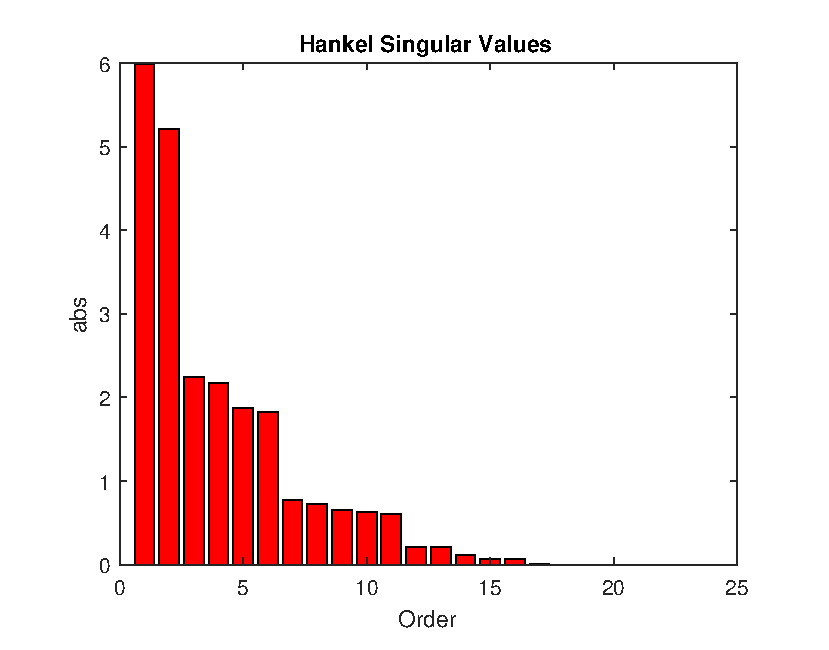
\includegraphics[width=10.8cm]{hsv_auto_h}  
\caption{HSV energy histogram of $K_H$ in GNSS-Dependent modes} 
\label{fig:APPlaunch}
\end{center}
\end{figure}

\section{Ground Control Station}
sdfsdfdsd

\begin{figure}[h]
\begin{center}
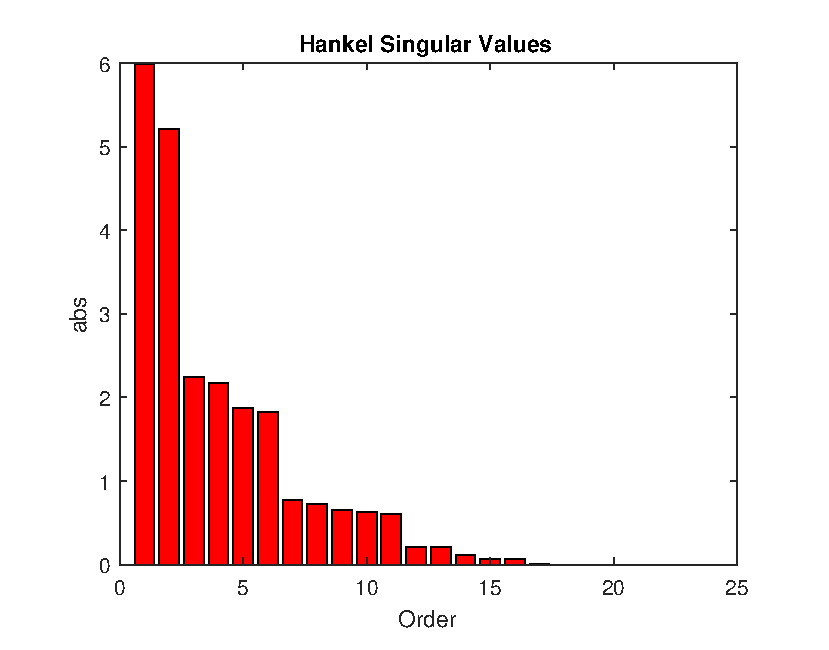
\includegraphics[width=10.8cm]{hsv_auto_h}  
\caption{HSV energy histogram of $K_H$ in GNSS-Dependent modes} 
\label{fig:hsv_auto_h}
\end{center}
\end{figure}

\section{Flight Tests}

\subsection{Stabilize Mode}

\subsubsection{LQI Controller}

\begin{figure}[H]
\begin{subfigure}{.5\linewidth}
\centering
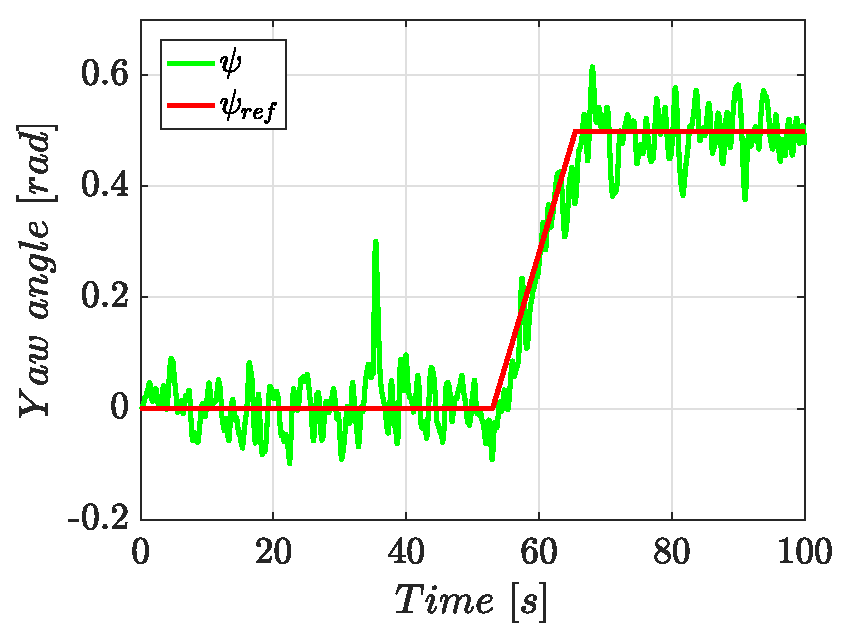
\includegraphics[width=7.0cm]{stabilize_psi_lqi_imp}
\caption{Rotation about $x$ axis, $J_{xx}$ experiment}
\label{fig:stabilize_psi_lqi_imp}
\end{subfigure}%
\begin{subfigure}{.5\linewidth}
\centering
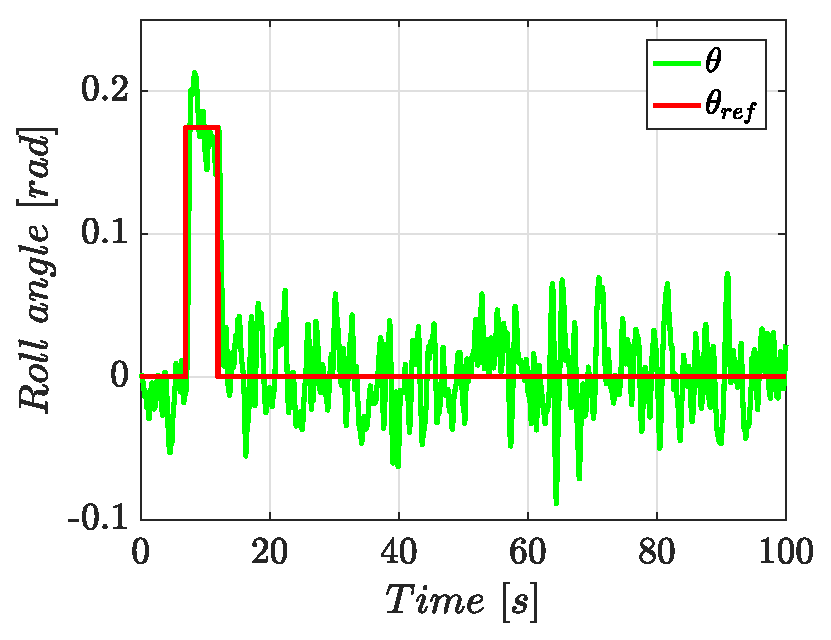
\includegraphics[width=7.0cm]{stabilize_theta_lqi_imp}
\caption{Rotation about $y$ axis, $J_{yy}$ experiment}
\label{fig:stabilize_theta_lqi_imp}
\end{subfigure}\\[1ex]
\begin{subfigure}{\linewidth}
\centering
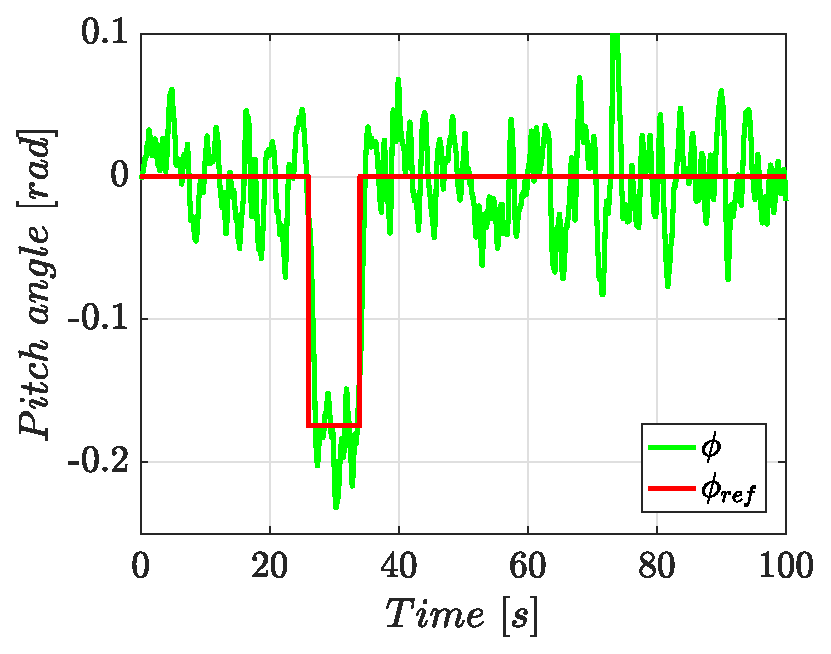
\includegraphics[width=7.0cm]{stabilize_phi_lqi_imp}
\caption{Rotation about $z$ axis, $J_{zz}$ experiment}
\label{fig:stabilize_psi_lqi_imp}
\end{subfigure}
\caption{Rotation about $x$, $y$ and $z$ axes during the bifilar pendulum experiments}
\label{fig:stabilize_lqi_imp}
\end{figure}


\subsubsection{$H_\infty$ Controller}

\begin{figure}[H]
\begin{subfigure}{.5\linewidth}
\centering
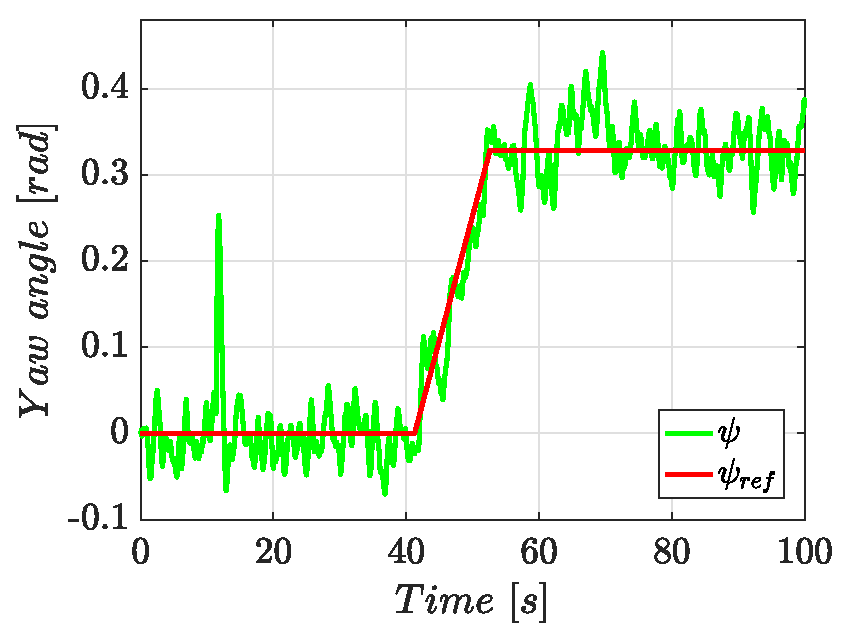
\includegraphics[width=7.0cm]{stabilize_psi_h_imp}
\caption{Rotation about $x$ axis, $J_{xx}$ experiment}
\label{fig:stabilize_psi_h_imp}
\end{subfigure}%
\begin{subfigure}{.5\linewidth}
\centering
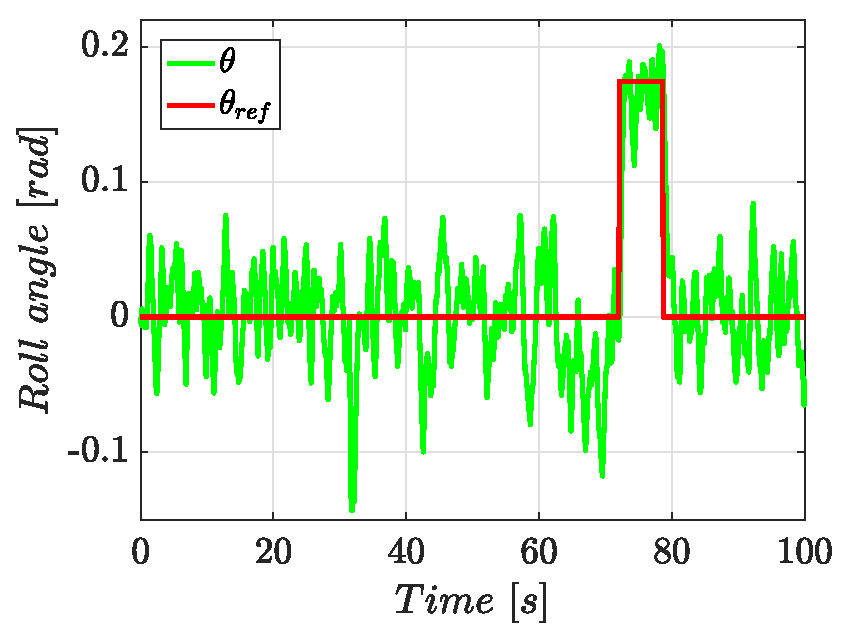
\includegraphics[width=7.0cm]{stabilize_theta_h_imp}
\caption{Rotation about $y$ axis, $J_{yy}$ experiment}
\label{fig:stabilize_theta_h_imp}
\end{subfigure}\\[1ex]
\begin{subfigure}{\linewidth}
\centering
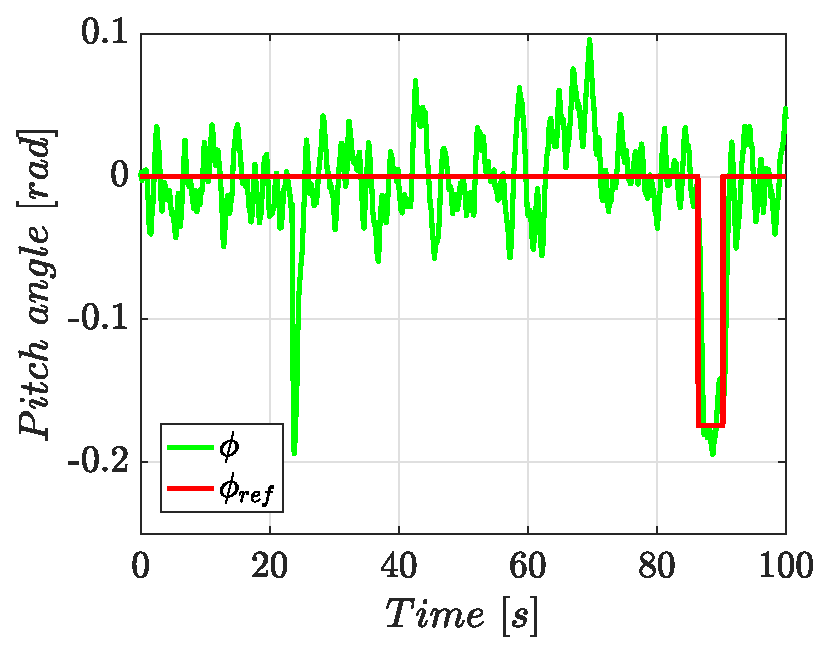
\includegraphics[width=7.0cm]{stabilize_phi_h_imp}
\caption{Rotation about $z$ axis, $J_{zz}$ experiment}
\label{fig:stabilize_psi_h_imp}
\end{subfigure}
\caption{Rotation about $x$, $y$ and $z$ axes during the bifilar pendulum experiments}
\label{fig:stabilize_h_imp}
\end{figure}


\subsection{Altitude Hold Mode}

\subsubsection{LQI Controller}

\begin{figure}[H]
\begin{subfigure}{.5\linewidth}
\centering
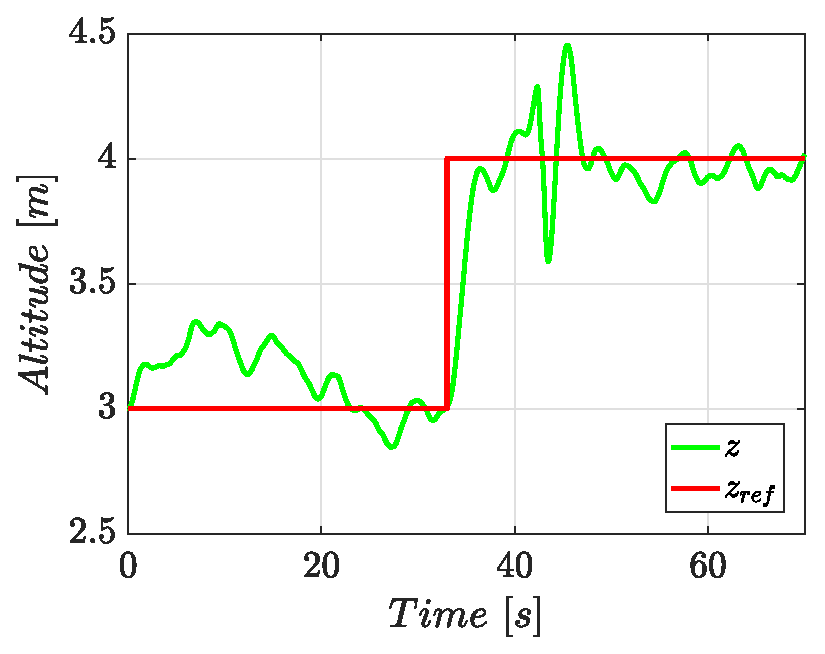
\includegraphics[width=7.0cm]{althold_z_lqi_imp}
\caption{Rotation about $x$ axis, $J_{xx}$ experiment}
\label{fig:althold_z_lqi_imp}
\end{subfigure}%
\begin{subfigure}{.5\linewidth}
\centering
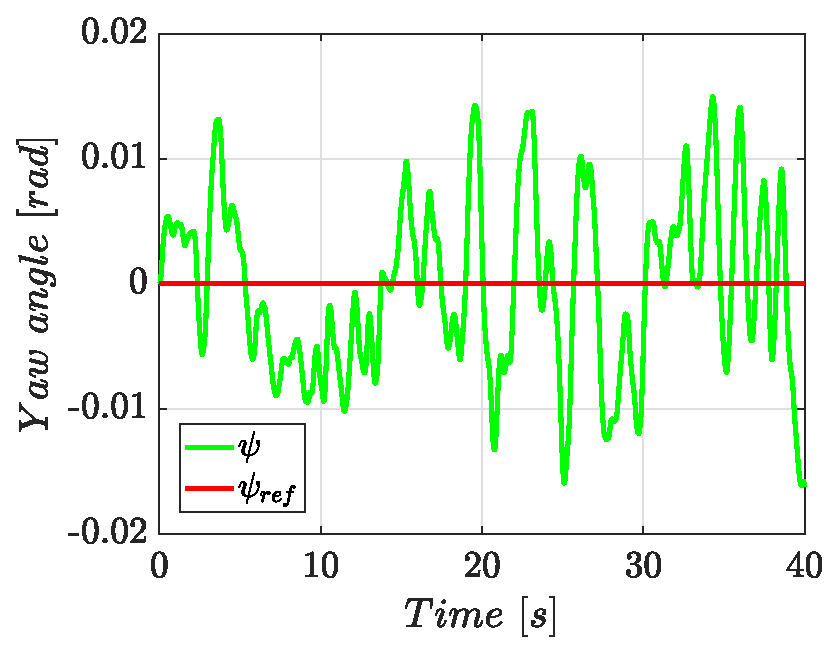
\includegraphics[width=7.0cm]{althold_psi_lqi_imp}
\caption{Rotation about $y$ axis, $J_{yy}$ experiment}
\label{fig:althold_psi_lqi_imp}
\end{subfigure}\\[1ex]
\begin{subfigure}{0.5\linewidth}
\centering
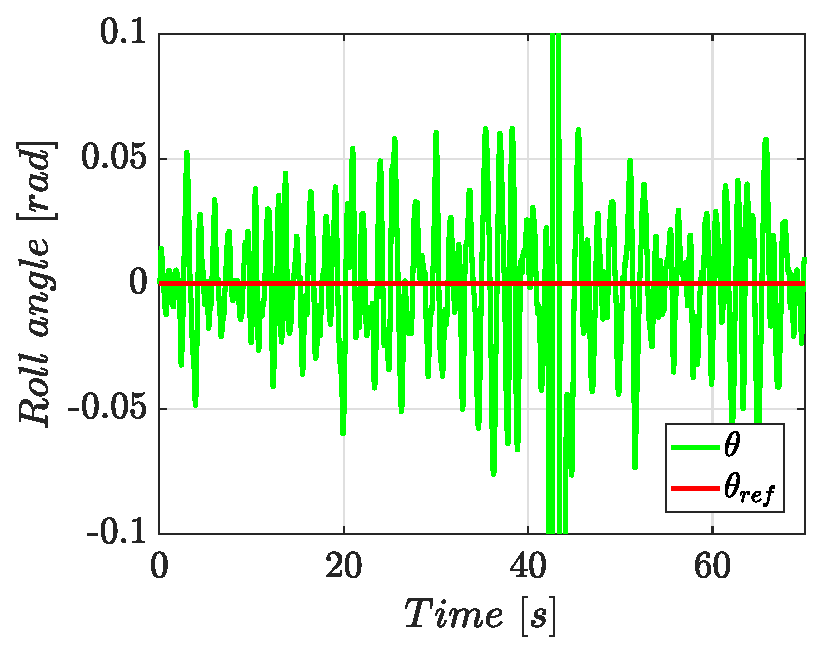
\includegraphics[width=7.0cm]{althold_theta_lqi_imp}
\caption{Rotation about $z$ axis, $J_{zz}$ experiment}
\label{fig:althold_theta_lqi_imp}
\end{subfigure}
\begin{subfigure}{0.5\linewidth}
\centering
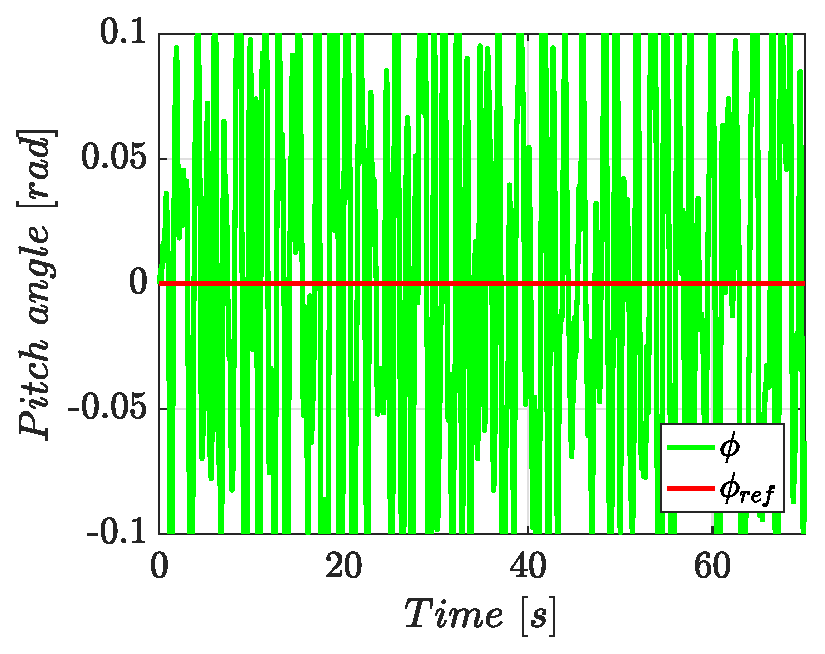
\includegraphics[width=7.0cm]{althold_phi_lqi_imp}
\caption{Rotation about $z$ axis, $J_{zz}$ experiment}
\label{fig:althold_phi_lqi_imp}
\end{subfigure}
\caption{Rotation about $x$, $y$ and $z$ axes during the bifilar pendulum experiments}
\label{fig:althold_lqi_imp}
\end{figure}


\subsubsection{$H_\infty$ Controller}

\begin{figure}[H]
\begin{subfigure}{.5\linewidth}
\centering
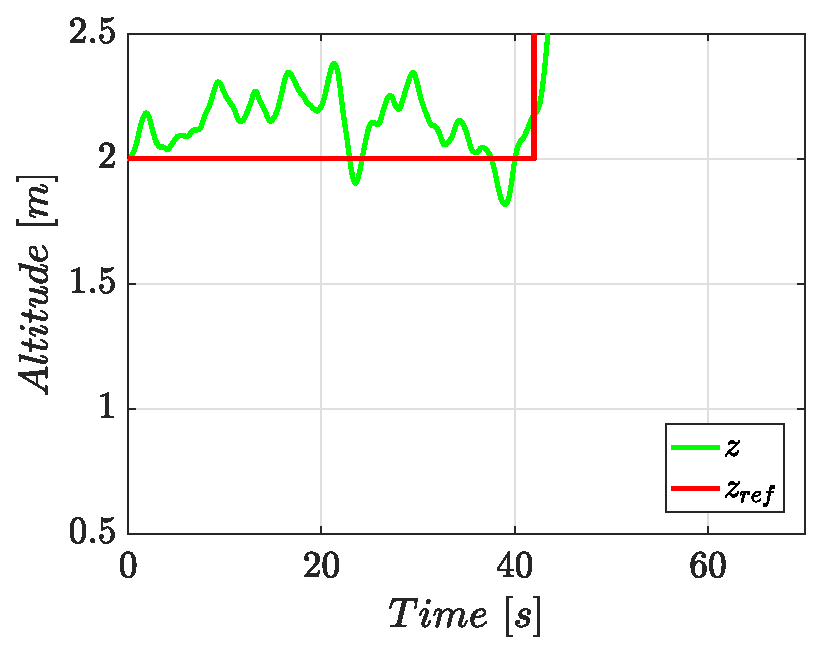
\includegraphics[width=7.0cm]{althold_z_h_imp}
\caption{Rotation about $x$ axis, $J_{xx}$ experiment}
\label{fig:althold_z_h_imp}
\end{subfigure}%
\begin{subfigure}{.5\linewidth}
\centering
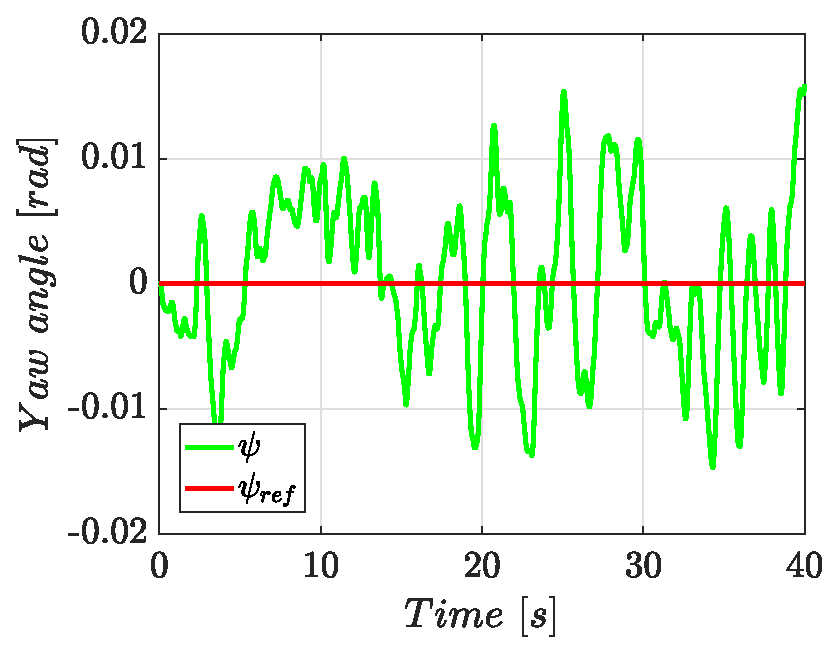
\includegraphics[width=7.0cm]{althold_psi_h_imp}
\caption{Rotation about $y$ axis, $J_{yy}$ experiment}
\label{fig:althold_psi_h_imp}
\end{subfigure}\\[1ex]
\begin{subfigure}{0.5\linewidth}
\centering
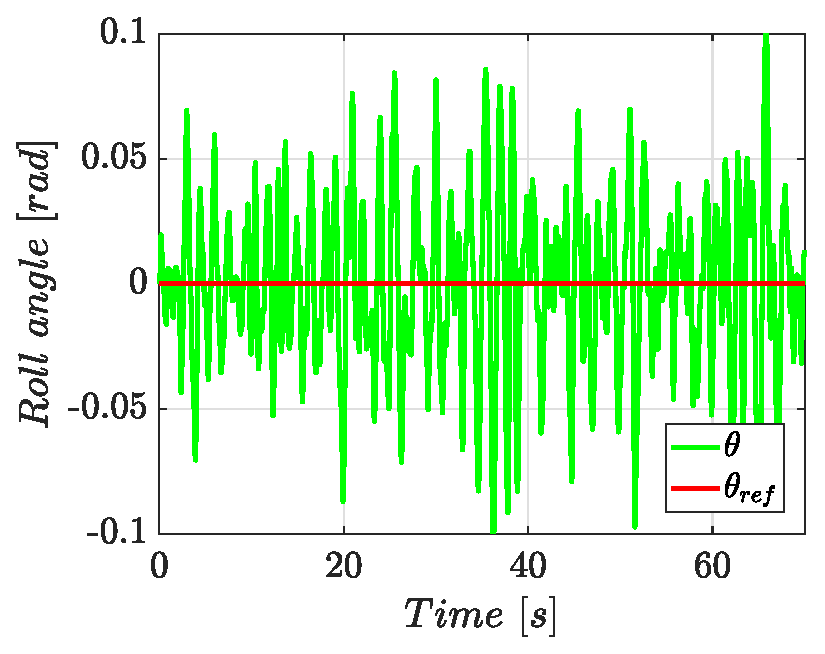
\includegraphics[width=7.0cm]{althold_theta_h_imp}
\caption{Rotation about $z$ axis, $J_{zz}$ experiment}
\label{fig:althold_theta_h_imp}
\end{subfigure}
\begin{subfigure}{0.5\linewidth}
\centering
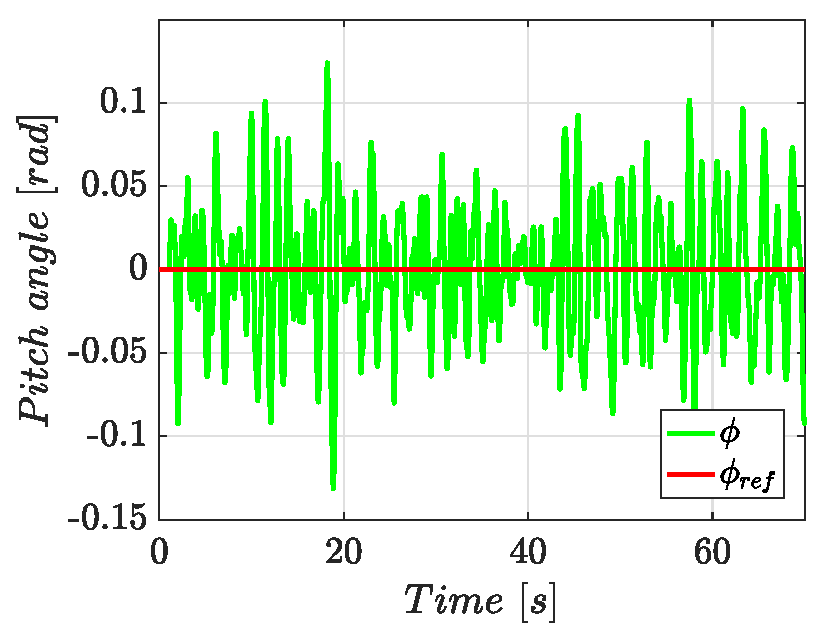
\includegraphics[width=7.0cm]{althold_phi_h_imp}
\caption{Rotation about $z$ axis, $J_{zz}$ experiment}
\label{fig:althold_phi_h_imp}
\end{subfigure}
\caption{Rotation about $x$, $y$ and $z$ axes during the bifilar pendulum experiments}
\label{fig:althold_h_imp}
\end{figure}



\subsection{GNSS-Dependent Mode}

\subsubsection{LQI Controller}

\begin{figure}[h]
	\begin{center}
	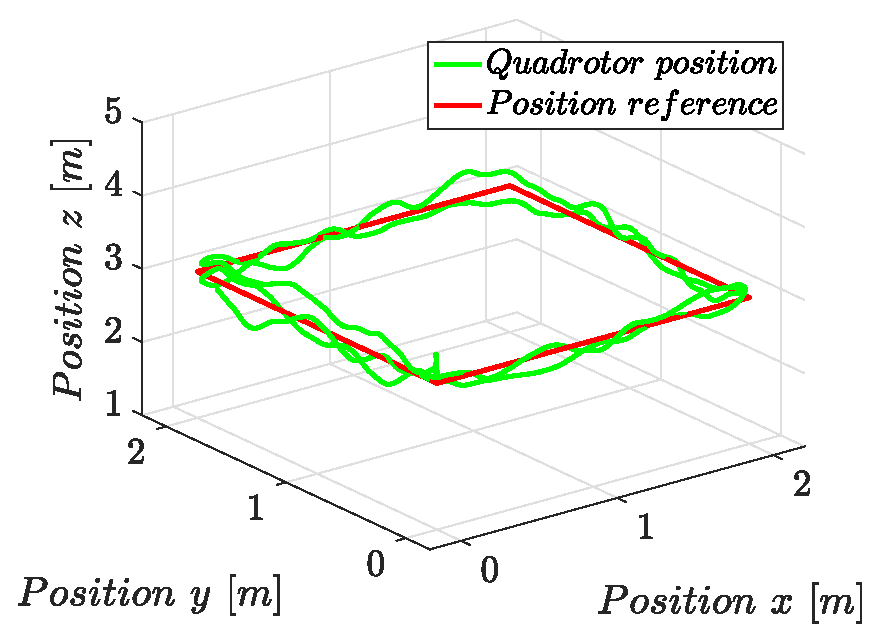
\includegraphics[width=0.8\textwidth]{auto_xyz_lqi_imp}
	\caption{Closed-loop of the controlled system with an $H_{\infty}$ controller.}
	\label{fig:auto_xyz_lqi_imp}
	\end{center}
	\end{figure}
	
\begin{figure}[H]
\begin{subfigure}{.5\linewidth}
\centering
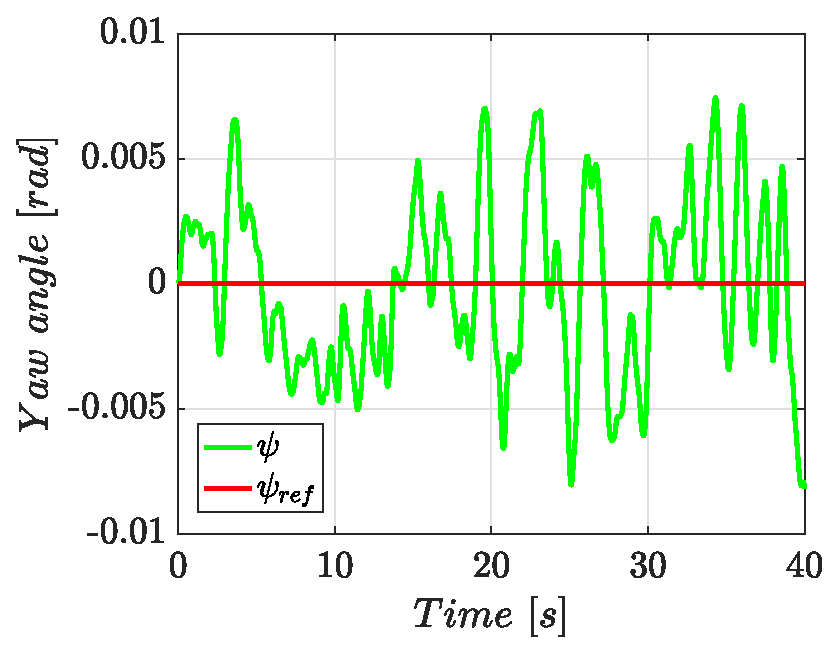
\includegraphics[width=7.0cm]{auto_psi_lqi_imp}
\caption{Rotation about $x$ axis, $J_{xx}$ experiment}
\label{fig:auto_psi_lqi_imp}
\end{subfigure}%
\begin{subfigure}{.5\linewidth}
\centering
\includegraphics[width=7.0cm]{auto_theta_lqi_imp}
\caption{Rotation about $y$ axis, $J_{yy}$ experiment}
\label{fig:auto_theta_lqi_imp}
\end{subfigure}\\[1ex]
\begin{subfigure}{\linewidth}
\centering
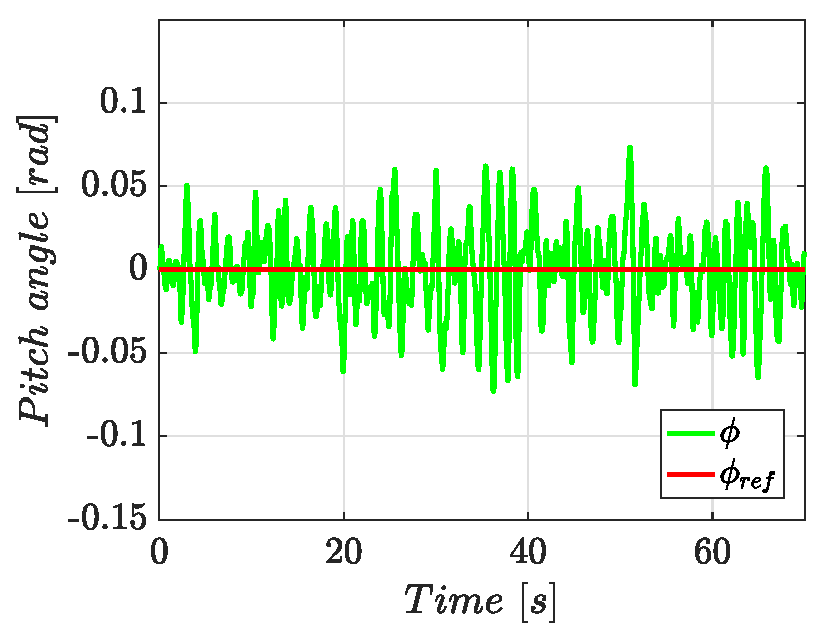
\includegraphics[width=7.0cm]{auto_phi_lqi_imp}
\caption{Rotation about $z$ axis, $J_{zz}$ experiment}
\label{fig:auto_psi_lqi_imp}
\end{subfigure}
\caption{Rotation about $x$, $y$ and $z$ axes during the bifilar pendulum experiments}
\label{fig:auto_lqi_imp}
\end{figure}


\subsubsection{$H_\infty$ Controller}

\begin{figure}[h]
	\begin{center}
	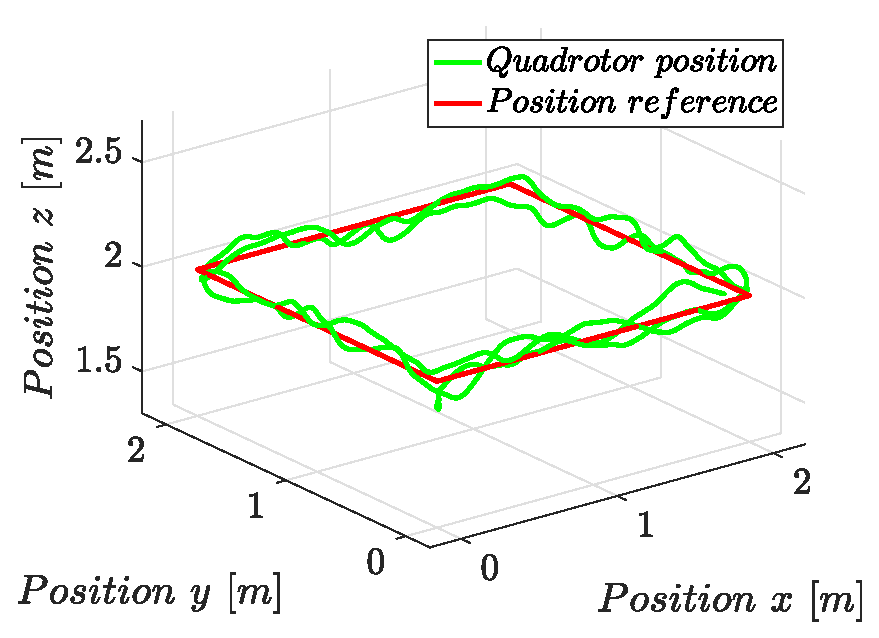
\includegraphics[width=0.8\textwidth]{auto_xyz_h_imp}
	\caption{Closed-loop of the controlled system with an $H_{\infty}$ controller.}
	\label{fig:auto_xyz_h_imp}
	\end{center}
	\end{figure}
	
\begin{figure}[H]
\begin{subfigure}{.5\linewidth}
\centering
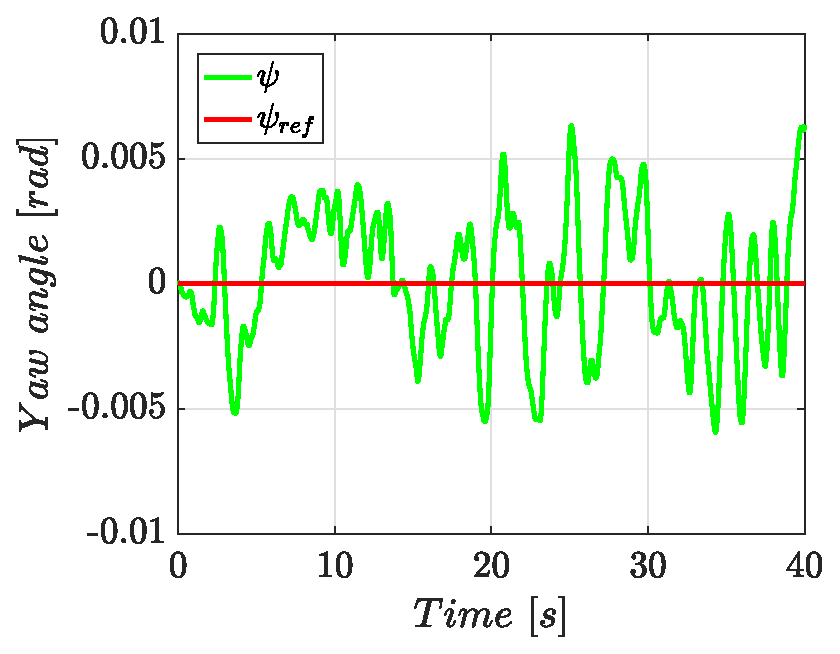
\includegraphics[width=7.0cm]{auto_psi_h_imp}
\caption{Rotation about $x$ axis, $J_{xx}$ experiment}
\label{fig:auto_psi_h_imp}
\end{subfigure}%
\begin{subfigure}{.5\linewidth}
\centering
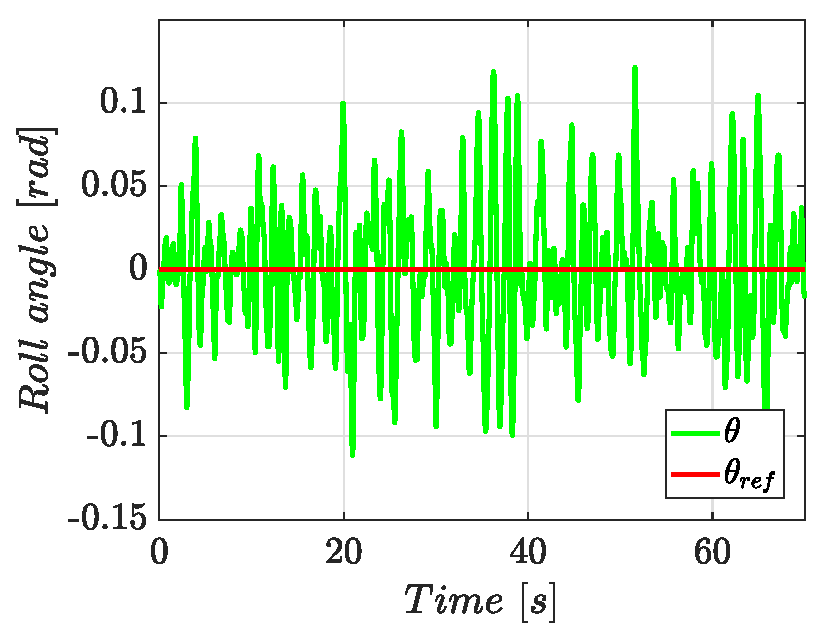
\includegraphics[width=7.0cm]{auto_theta_h_imp}
\caption{Rotation about $y$ axis, $J_{yy}$ experiment}
\label{fig:auto_theta_h_imp}
\end{subfigure}\\[1ex]
\begin{subfigure}{\linewidth}
\centering
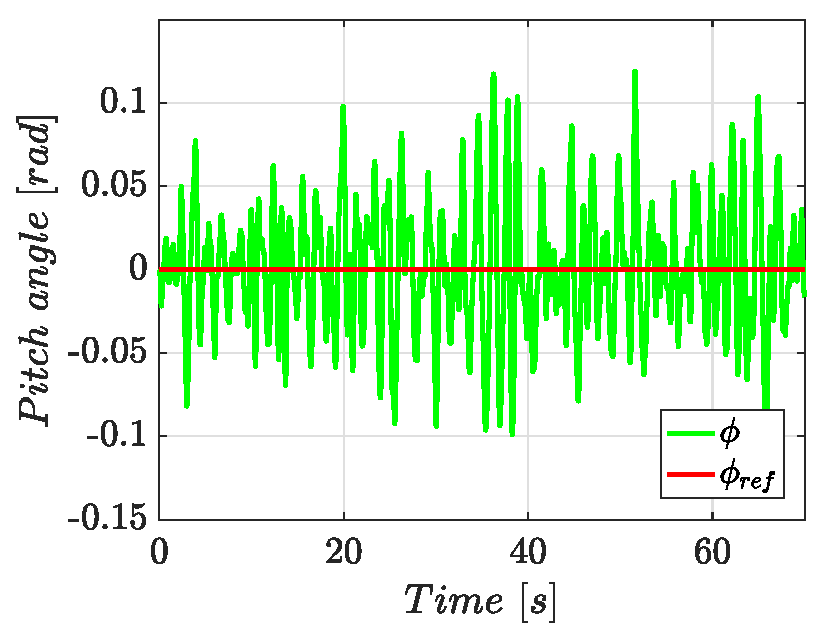
\includegraphics[width=7.0cm]{auto_phi_h_imp}
\caption{Rotation about $z$ axis, $J_{zz}$ experiment}
\label{fig:auto_psi_h_imp}
\end{subfigure}
\caption{Rotation about $x$, $y$ and $z$ axes during the bifilar pendulum experiments}
\label{fig:auto_h_imp}
\end{figure}




\section{Conclusions}
rgrgrgtrgrtgr